\documentclass[11pt,letterpaper]{article}
\usepackage[top=1in,bottom=1in,left=1in,right=1in]{geometry}
\usepackage[numbers]{natbib}      % http://merkel.zoneo.net/Latex/natbib.php
\usepackage{lmodern}
\renewcommand\familydefault{\sfdefault} 
\usepackage[T1]{fontenc}

%\bibpunct{(}{)}{;}{a}{,}{,}
\usepackage{chngpage}
\usepackage{stmaryrd}
\usepackage{amssymb}
\usepackage{amsmath}
\usepackage{amsthm}
\usepackage{graphicx}
\usepackage{lscape}
\usepackage{subfigure}
\usepackage{parskip}
\usepackage[usenames,dvipsnames]{color}
\usepackage{indentfirst}
\definecolor{myblue}{rgb}{0,0.1,0.6}
\definecolor{mygreen}{rgb}{0,0.3,0.1}
\usepackage[colorlinks=true,linkcolor=black,citecolor=mygreen,urlcolor=myblue]{hyperref}
\newcommand{\bocomment}[1]{\textcolor{Bittersweet}{[#1 -BTO]}}
\newenvironment{itemizesquish}{\begin{list}{\labelitemi}{\setlength{\parskip}{0.6cm}\setlength{\itemsep}{0em}\setlength{\labelwidth}{2em}\setlength{\leftmargin}{\labelwidth}\addtolength{\leftmargin}{\labelsep}}}{\end{list}}
\newcommand{\norm}[1]{\left\lVert#1\right\rVert}
\newcommand{\ignore}[1]{}

\theoremstyle{definition}
\newtheorem{question}{Question}[section]

\setlength{\parindent}{30pt}
\linespread{1}

\title{
Protein sequence classification using neighbor-joining\\
   CMSC 701 Final report
}

\author{
	Khanh Nguyen and Ugur Koc
}

\begin{document}
\maketitle

\section{Introduction}

Neighbor-joining is a widely used algorithm for reconstructing phylogenetic trees from evolutionary distance data. The method takes a greedy bottom-up approach, iteratively joining pairs of taxonomic units that minimizes pre-computed distances. In this work, we present our C++ implementation of the algorithm. We compare the running time of the implementation with other popular packages. In addition, we also provide a benchmark on our implementation for computing the distance matrix between sequences. We found that BLAH BLAH.

\section{Background}

\subsection{Hierarchical clustering}

\subsection{Phylogenetic trees}

\begin{figure}[h]
  \centering
  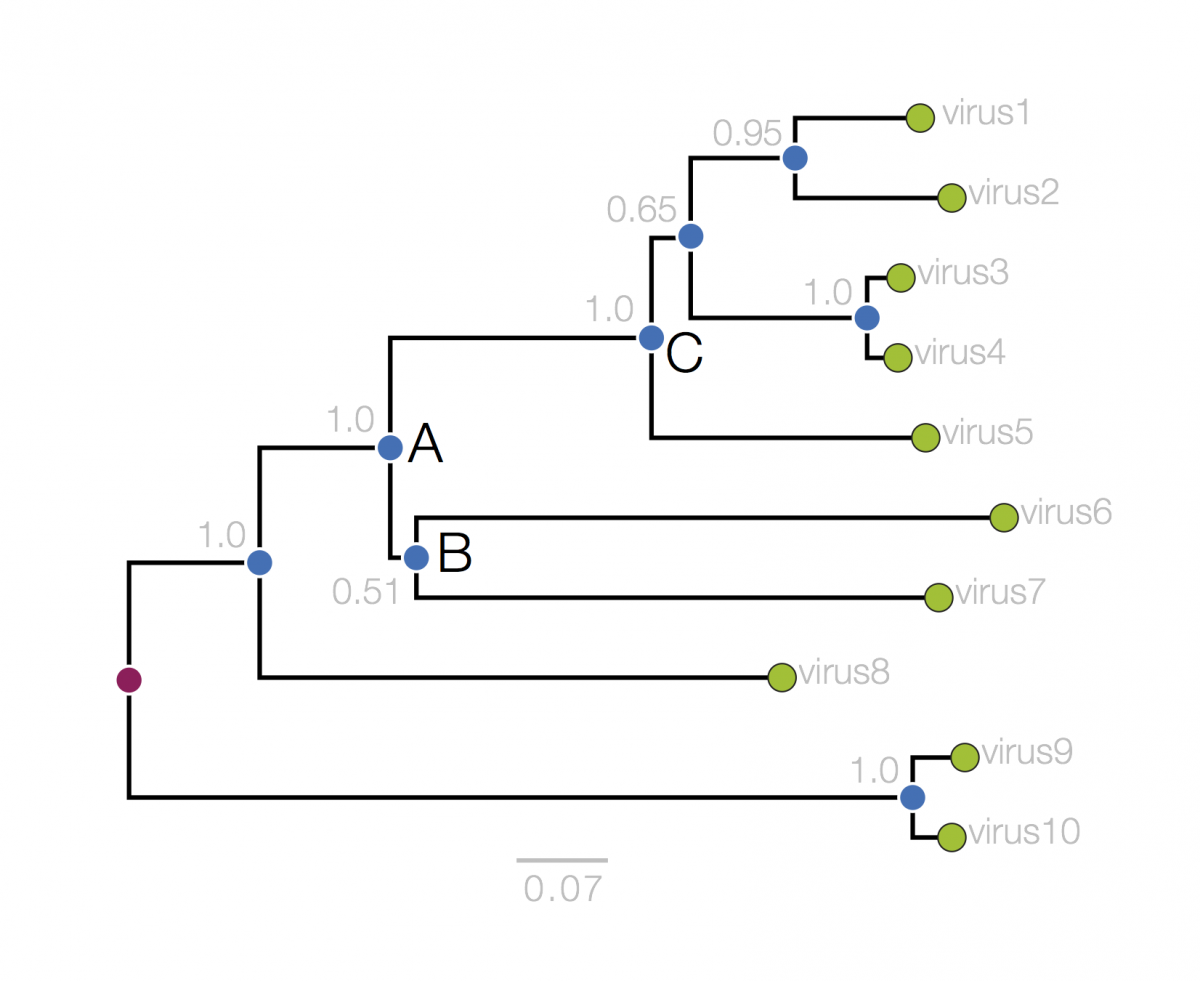
\includegraphics[width=0.6\textwidth]{phylogram_1a.png}
  \caption{An example of phylogenetic tree.}
  \label{fig:phytree}
\end{figure}

Phylogenetic trees are branching diagrams that show the evolutionary relationships between biological species. A weighted phylogenetic tree, with weights associated with its edges, captures the notion of genetic distances between species. Hence, looking at a weighted phylogenetic tree, we understand not only \textit{how} but also \textit{how much} they relates or differs from one another. Figure \ref{fig:phytree} \footnote{Image taken from \url{http://epidemic.bio.ed.ac.uk/how_to_read_a_phylogeny}} features a artificial phylogenetic tree of 10 viruses. Each virus is represented by a leave in the tree. Each internal node marks a milestone when a genetic divergence occurs. Notice that the lengths of the horizontal lines represents time periods. For example, we can see that the divergence between virus 1 and virus 2 occurs before the divergence between virus 3 and 4. Different phylogenetic trees may choose to represent different types of genetic distances. In this example, the number assigned to each edge is the proportion of substitutions occurring on a sequence (the number of substitutions divided by the length of the sequence). 

%\subsection{Distance matrix}

\section{Method}

\subsection{Neighbor-joining algorithm}

In this report, we consider the problem of constructing a phylogenetic tree from a set of protein sequences. From a data mining or machine learning perspective, this problem can be framed as hierarchical clustering problem. There are many approaches to tackle this problem. Although statistical approaches such as maximum likelihood methods have been employed to build complex evolution model, classical approaches such as the neighbor-joining algorithm has the advantage of being easy to implement and scalable to large datasets. Our focus in this report is on the neighbor-joining algorithm~\cite{saitou1987neighbor}. 

TODO: Khanh 
Neigh-joining algorithm takes 


\subsection{Computing distance matrix}

Neigbor-joining algorithm is deterministic, i,e, given a distance matrix it will always produce the same phylogenetic three. Therefore achieving accurate results highly depend on the model of evaluation, i,e, distance matrix.
We have used two packages to compute distance matrix. For already aligned sequences, we used the package emboss\footnote{\url{http://emboss.sourceforge.net/apps/release/6.6/emboss/apps/distmat.html}} \cite{rice2000emboss}. Emboss has \textit{distmat} program, which computes distance matrix for already aligned sequences. We wrote a wrapper script in perl to call this program and then post process it's output in order to put it in the format of input distance matrix of our NJ implementation (see \textit{aligntodist.pl} script in source code).

\textit{distmat} has tree different multiple substitution correction methods implemented for aligned proteins sequences. They are Uncorrected, Jukes-Cantor~\cite{jukes1969evolution}, and Kimura Protein~\cite{kimura1980simple}. 

To compute distance matrix for a set of protein sequences we used \textit{protdist} program from phylib\footnote{\url{http://evolution.genetics.washington.edu/phylip.html}} package~\cite{plotree1989phylip}. We slightly modified the source code in order to have the output in required format and we removed the unnecessary functionality which does not matter for this project (see \textit{protdist.c} source file for details).

\textit{protdist} has five method for amino-acid substitutions. They are Dayhoff PAM matrix~\cite{kosiol2005different}, Jones-Taylor-Thornton model~\cite{jones1992rapid}, PMB (Probability Matrix from Blocks) model~\cite{veerassamy2003transition}, Kimura's distance~\cite{kimura1983rare}, and Categories distance\footnote{See \url{http://evolution.genetics.washington.edu/phylip.html}}

\section{Experiment}

To evaluate the effectiveness and the efficiency of our implementations, we conducted a set of experiments. 

We first aimed at generating accurate phylogenetic tree trying out different evaluation models when generating the distance matrix. We then compared our results with some other popular implementations of neighbor-joining algorithm. 

In these experiments, effectiveness refers to the accuracy of the phylogenetic tree produced at the end, i.e. how close/similar the tree to the ground truth (we take the results in \cite{khafif2014identification} as the ground truth), and the efficiency refers to the computation time. 

\subsection{Data}

In all experiments, we used the data and results given by Khafif et. al~\cite{khafif2014identification}. 

TODO: do we have time to experiment on other data?. 

\subsection{Results}

\subsubsection{Study 1; Generating accurate phylogenetic tree}

Here we compare effectiveness and efficiency of methods implemented in \textit{distmat} and \textit{protdist}. 

\textbf{Performance of \textit{distmat} methods}. Figure~\ref{fig:phytree} and~\ref{fig:phytree} show time computation times and the phylogenetic tree accuracies for the methods implemented in \textit{distmat} respectively. TODO

\textbf{Performance of \textit{protdist} methods}. Figure~\ref{fig:phytree} and~\ref{fig:phytree} show time computation times and the phylogenetic tree accuracies for the methods implemented in \textit{protdist} respectively. TODO 

\subsubsection{Study 2; Comparing with other neighbor-joining implementations}
 
TODO: Khanh 

\subsubsection{Comparing distance matrix methods}



\bibliographystyle{plain}
\bibliography{report}

\end{document}






